% New HW24 solution, checked numerically with build_hw24_solution.py.
% This expanded assignment is distinct from the legacy Lesson-24 algebra sheet.
% Private instructor material. Numerical tables are generated, not hand-entered.
\subsection*{Review notes and reproducibility}
This solution follows the current local \texttt{homework/markdown/HW24.md},
confirmed by the instructor on November 2, 2026: depletion;
reactivity and poison cross sections; three-batch cycle estimates;
and the infinite-dilution mistake. The starter comments specify the
301-point fit grid; numerical bounds and sensitivity checks support the
instructor reference. The Gd addition is an isotope number density in fuel;
it leaves the original uranium and oxygen inventories unchanged. It is not
a natural-Gd or gadolinia mass fraction.

Run \texttt{python build\_hw24\_solution.py} from this directory, then
\texttt{make} for the full HW01--28 manual, or
\texttt{make hw24\_review.pdf} for the standalone copy. The executed
\texttt{hw24\_solution.ipynb} contains the same numerical source and its
outputs. The retained CSV tables and \texttt{provenance.json} in
\texttt{data/hw24/} include solver settings, package versions, source hashes,
unrounded results, and verification evidence. All reactivities below are
dimensionless unless a percent or pcm unit is shown explicitly.

The numerical reference uses the assigned starter grid augmented by
0.01-day sampling during the first 30 days and about 0.208-day sampling
afterward. Fits use linear interpolation onto exactly 301 evenly spaced
points from 1 to 40 MWd/kg. Extrema include both endpoints and all relevant
interpolation knots. Digits retained in generated tables identify the
calculation; they do not measure physical model accuracy.

\subsection*{Common inputs from the current assignment}
Use the Lesson 24 notebook and \texttt{ne630\_depletion}, with NumPy, SciPy,
pandas, and Matplotlib. Both cells use $V_m/V_f=2$, water density
$0.7$ g/cm$^3$, moderator/fuel flux ratios $(1,1,1.16)$, and
\texttt{nonleakage=1}; leakage is applied separately as $\rho_L=0.05$.
Use 4\% U-235 by initial uranium mass, UO$_2$ density 10.4 g/cm$^3$,
fuel diameter 0.82 cm, and initial Gd-157 loadings of 0 or $10^{18}$
atoms/cm$^3$ fuel. All other tracked nuclides initially vanish, including
I/Xe and Pm/Sm. Use model 3 with explicit poisons, constant
$P^{\prime\prime\prime}=300$ W/cm$^3$ fuel, spectrum $(0.35,0.55,0.10)$,
and U-238 shielding \texttt{UO2Shielding(10.4,0.82)}. Irradiate from
0 to 3.5 full-power years, with $\mathrm{YEAR}=365.25\,\mathrm{DAY}$.
Use the initial HM density excluding Gd, the module burnup, and
\texttt{neutronics("rate\_ratio")["rho"]}. Three equal-mass batches
have equal weights and burnup increments. The reference reproduces
the starter time grid before adding the finer samples documented above.

\clearpage
\subsection*{(1) Deplete the two pincells}
\textbf{Problem.} Run both cases using the shielded U-238 data. Confirm
constant power and burnup proportional to elapsed time. Plot flux versus
time, report its initial and final values for each case, and explain why
fixed power does not imply fixed flux.

\begin{draftsolution}
Using the module's integer molar masses and 4\% uranium mass enrichment,
\[
 M_U=\left(\frac{0.04}{235}+\frac{0.96}{238}\right)^{-1},\qquad
 \rho_{\mathrm{HM},0}=0.0104\frac{M_U}{M_U+32}
 =0.00916685263\ \mathrm{kg/cm^3}.
\]
Both cases have the same initial heavy-metal mass. With $t$ in seconds,
\[
 B(t)=\frac{300t}{8.64\times10^{10}\rho_{\mathrm{HM},0}},\qquad
 \frac{dB}{dt_{\mathrm{days}}}=0.0327266\ \mathrm{MWd/(kg\,day)}.
\]
Thus 3.5 full-power years are 1278.375 days and give
$B=41.83688$ MWd/kg in both cases. The computed power is
300 W/cm$^3$ throughout. Fixed power imposes the fission rate,
\[
 \phi(t)=\frac{P^{\prime\prime\prime}}
 {\kappa\sum_i N_i(t)\bar\sigma_{fi}},
 \qquad \kappa=200\ \mathrm{MeV/fission}.
\]
For either Gd loading, the shielded-case flux starts at
$1.499582\times10^{14}$ and ends at
$2.559859\times10^{14}$ n/cm$^2$/s. The flux rises to compensate for the
evolving fission inventory.

There is an exact structural reason that Gd does not change these fluxes
in this exercise: it has no fission cross section, does not feed actinides,
and cannot change the prescribed spectrum or the imposed power. The
actinide equations and power normalization are independent of its density.
An actual spectrum and power distribution would respond to poison loading.
\end{draftsolution}
\begin{center}
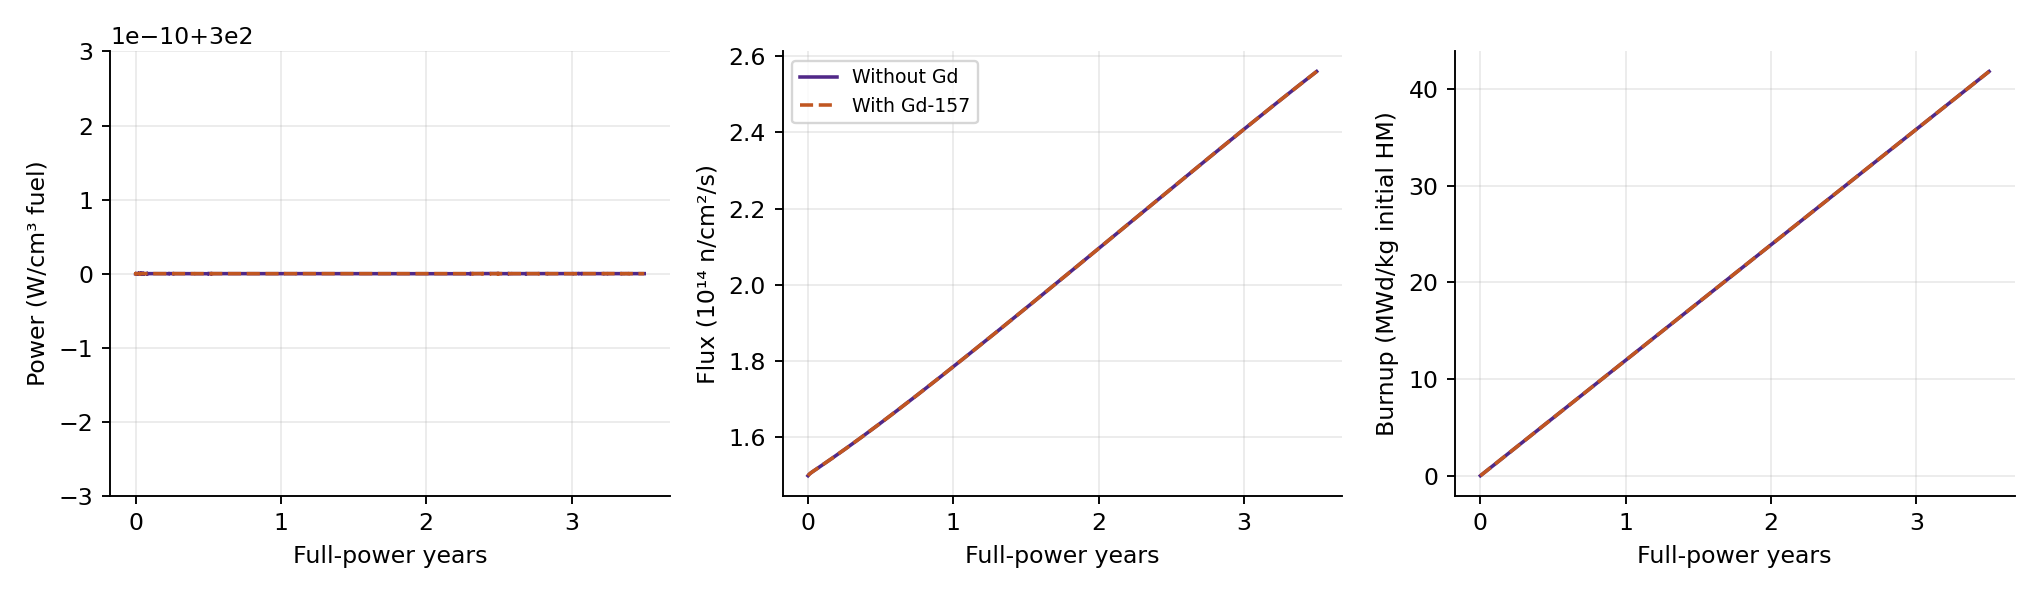
\includegraphics[width=\textwidth]{hw24_power_flux_burnup.png}
\end{center}

\clearpage
\subsection*{(2) Reactivity and macroscopic poison cross sections}
\textbf{Problem.} Plot reactivity over 0--40 MWd/kg and macroscopic
Gd-157 and Xe-135 absorption over the first 30 days for the Gd-bearing case.

\begin{draftsolution}
The plotted cross sections are spectrum-averaged macroscopic absorption:
\[
 \overline{\Sigma}_{a,i}(t)=N_i(t)\,10^{-24}
 \sum_{g\in\{F,I,T\}}w_g\sigma_{a,i,g}\quad[\mathrm{cm^{-1}}],
 \qquad (w_F,w_I,w_T)=(0.35,0.55,0.10).
\]
The microscopic cross sections and spectrum are fixed. Their macroscopic
counterparts evolve because the number densities change. Both nuclides
are nonfissioning in this chain, so absorption equals capture for these
plots. The group-weighted microscopic values are approximately
19,236.47 b for Gd-157 and 264,365.46 b for Xe-135.

The following endpoint values are all in cm$^{-1}$:
\begin{center}\small
\begin{tabular}{lrrrr}
\toprule
Case & Gd-157, day 0 & Gd-157, day 30 & Xe-135, day 0 & Xe-135, day 30 \\
\midrule
With Gd-157 & $1.92365\times10^{-2}$ & $1.02107\times10^{-5}$ & 0 & $2.65585\times10^{-3}$ \\
\bottomrule
\end{tabular}
\end{center}

For the Gd-bearing case, Gd macroscopic absorption starts near
0.01924 cm$^{-1}$ and falls quickly as Gd is consumed. Xenon starts at zero and builds through the I-135 precursor
and direct fission yield; it approaches a slowly changing balance between
production, radioactive decay, and neutron capture. The plotted Xe absorption is for the Gd-bearing case; it also equals
the non-Gd result to numerical accuracy because Gd cannot change the
actinide or flux histories under the prescribed-spectrum fixed-power
assumptions. The resulting competition between decreasing Gd absorption
and increasing Xe absorption explains the startup reactivity behavior.

The extrema over the closed interval $0\le B\le40$ MWd/kg are:
\begin{center}\small
\begin{tabular}{lrrrr}
\toprule
Shielded case & $\rho(0)$ & Min & Max & Swing (pcm) \\
\midrule
Shielded, no Gd & 0.274681 & 0.085500 & 0.274681 & 18918 \\
Shielded, Gd & 0.148613 & 0.085500 & 0.251014 & 16551 \\
\bottomrule
\end{tabular}
\end{center}

The unpoisoned maximum occurs at startup. With Gd, the maximum is near
$B=0.685$ MWd/kg, or 20.92 full-power days. Both minima occur at
$B=40$ MWd/kg. Gd reduces initial excess reactivity by about 12,607 pcm,
but reduces the full 0--40 peak-to-trough swing by only about 2367 pcm:
the curve rebounds as Gd burns out. It does not flatten the entire
depletion history.

At the initial shielded flux, the Gd absorption cross section condensed
on the assigned spectrum is about 19,236.5 b, giving an initial burnout
half-time of about 2.78 days. More exactly,
\[
 N_{157}(t)=N_{157}(0)
 \exp[-\bar\sigma_{a,157}\,10^{-24}\mathcal F(t)],
 \qquad \mathcal F(t)=\int_0^t\phi(t')\,dt'.
\]
The independently evaluated exponential agrees with the integrated Gd
inventory. Xenon and samarium buildup add negative reactivity while Gd
burnout adds positive reactivity. In this loading the Gd effect initially
dominates; later, depletion drives the decline. At 1 MWd/kg, roughly
30.56 days, only about $4.6\times10^{-4}$ of the initial Gd remains.
The later actinide histories coincide and the post-startup fits nearly
coincide. Small remaining fit differences are resolved numerically but
are immaterial at the intended reporting precision.
\end{draftsolution}
\begin{center}
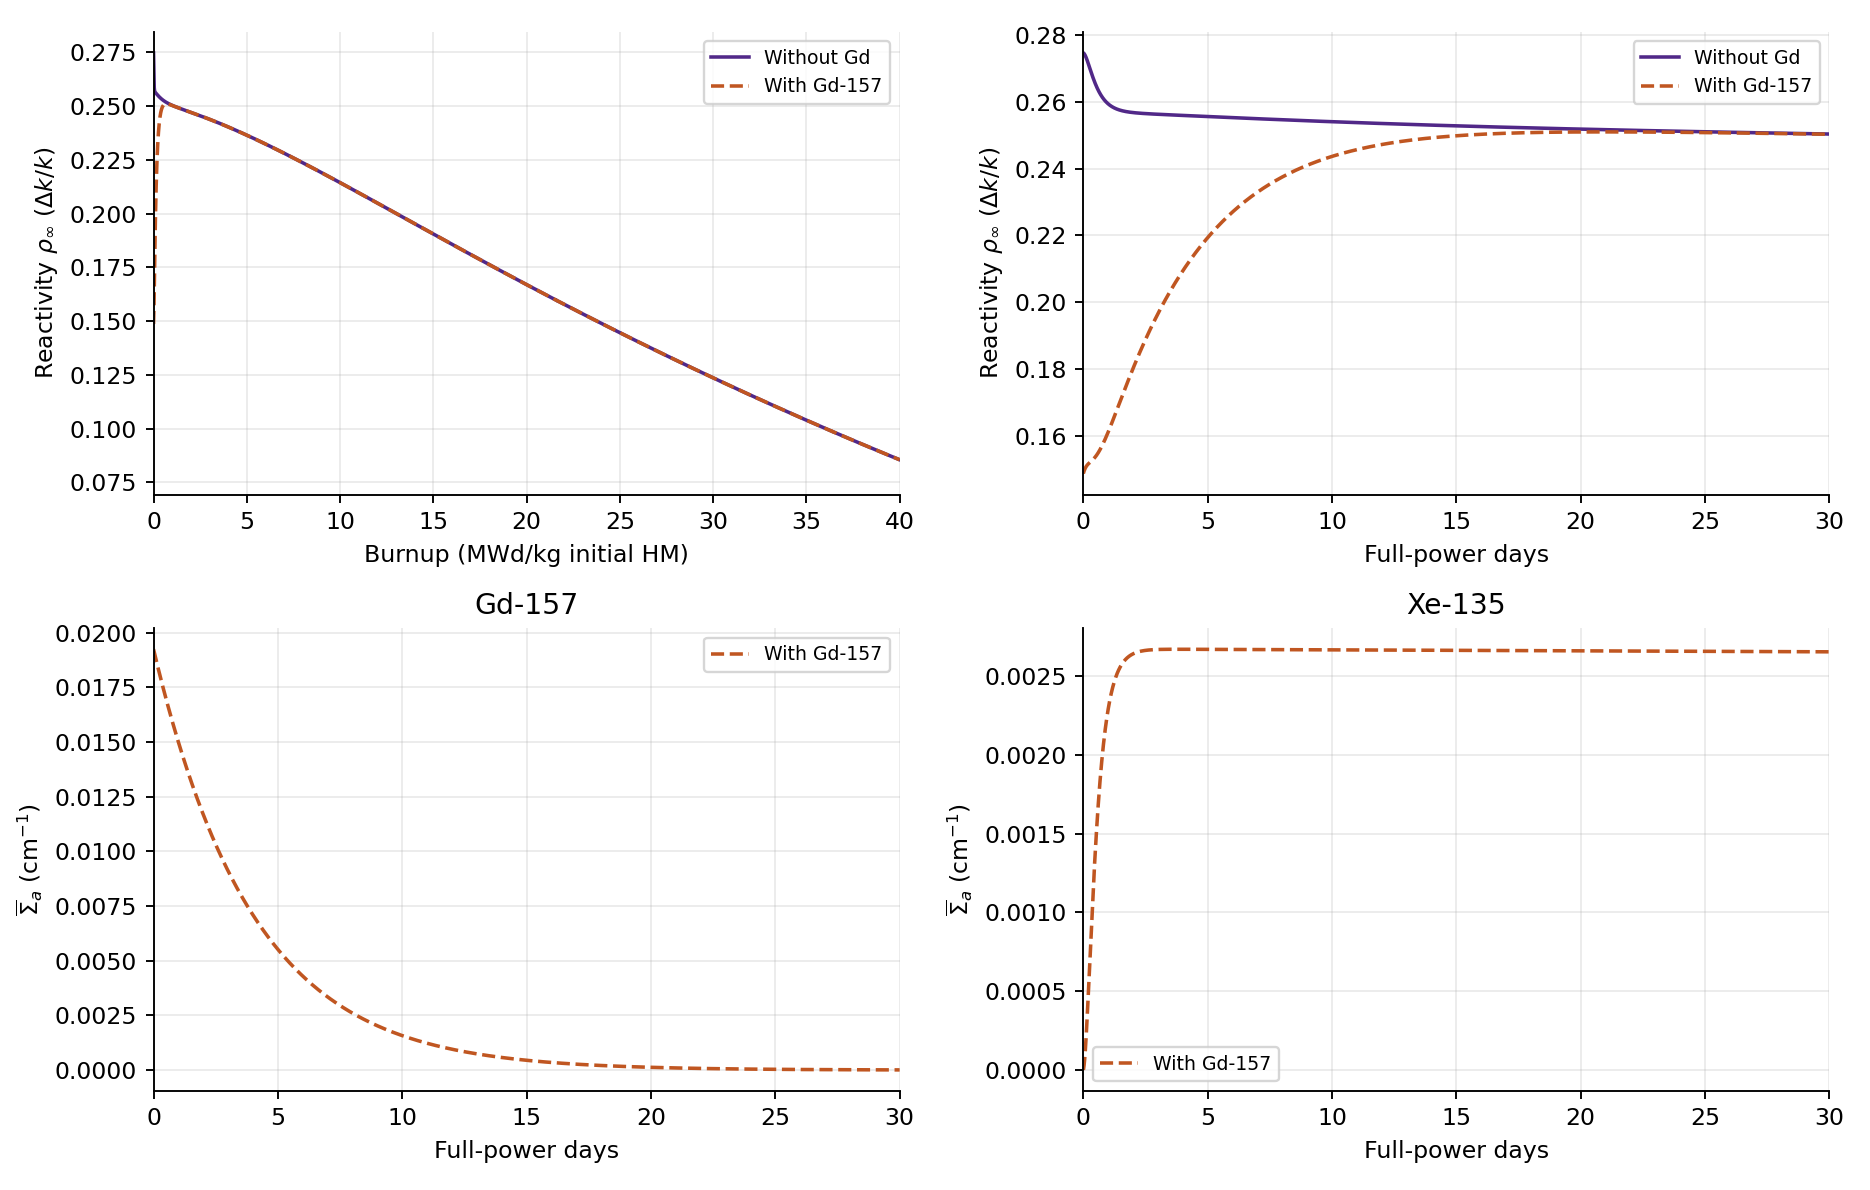
\includegraphics[width=\textwidth]{hw24_startup.png}
\end{center}


\clearpage
\subsection*{(3) Fit and three-batch cycle estimate}
\textbf{Problem.} For each case, fit $\rho_\infty(B)=\rho_0-aB$ on
301 evenly spaced points from 1 to 40 MWd/kg, addressing the early peak
or dip. At equilibrium EOC the batch burnups are $B_c$, $2B_c$, and
$3B_c$. Set their average reactivity minus 0.05 to zero; derive and
evaluate $B_c$, $B_d=3B_c$, and the cycle length in full-power days.

\begin{draftsolution}
Fit $\rho_\infty(B)=\rho_0-aB$ on the 301 evenly spaced burnup points
from 1 to 40 MWd/kg specified in the starter code comments. Starting at 1 MWd/kg
(about 30.56 full-power days) bypasses the startup Xe dip and Gd burnout
peak. The fitted intercept extends this post-startup trend back to zero
burnup; it is not the fresh-fuel reactivity.

For equal batch weights at EOC,
\[
 0=\rho_0-\frac{a}{3}(B_c+2B_c+3B_c)-\rho_L
 =\rho_0-2aB_c-\rho_L.
\]
Consequently,
\[
 \boxed{B_c=\frac{\rho_0-\rho_L}{2a}},\qquad
 \boxed{B_d=3B_c},\qquad
 \boxed{t_c=\frac{10^6\rho_{\mathrm{HM},0} B_c}{300}
        =30.55618 B_c\ \mathrm{days}}.
\]
The multiplier $10^6$ converts MW to W; the day unit is already contained
in MWd/kg. No additional factor of 86400 belongs in this day expression.

The fit results for the two shielded histories and the unshielded non-Gd
history are collected here; the $I_\infty$ row is interpreted in part (4). Slopes have units
$(\mathrm{MWd/kg})^{-1}$.
\begin{center}\small
\begin{tabular}{lrrrr}
\toprule
Case & $\rho_0$ & $-a$ & RMS (pcm) & Max (pcm) \\
\midrule
Shielded, no Gd & 0.256699 & -0.00439446 & 177.6 & 458.0 \\
Shielded, Gd & 0.256698 & -0.00439442 & 177.7 & 457.9 \\
$I_\infty$, no Gd & -0.815447 & 0.01959103 & 11276.5 & 48897.0 \\
\bottomrule
\end{tabular}
\end{center}

\begin{center}\small
\begin{tabular}{lrrrr}
\toprule
Case & $B_c$ & $B_d$ & Days & LRM assumptions \\
\midrule
Shielded, no Gd & 23.518 & 70.554 & 718.62 & satisfied \\
Shielded, Gd & 23.518 & 70.555 & 718.63 & satisfied \\
$I_\infty$, no Gd & 22.088 & 66.263 & 674.92 & INVALID \\
\bottomrule
\end{tabular}
\end{center}

Burnups in the cycle table are MWd/kg initial HM. Both shielded fits have
$a>0$ and $\rho_0>0.05$. They predict approximately 23.52 MWd/kg per
cycle, 70.55 MWd/kg discharge, and 718.6 full-power days.

The shielded EOC burnups are approximately
$(23.52,47.04,70.55)$ MWd/kg. Only the youngest batch lies inside the
1--40 fit interval; the other two also exceed the computed history's
41.84 MWd/kg endpoint. These formal limiting cycles are substantial
extrapolations. They are not supported fuel-use predictions for the 4\%
fuel. An optional appendix compares the nonlinear and linear models
within the available history using a 10 MWd/kg cycle; this is a check
beyond the revised assignment's required parts.

RMS residuals near 178 pcm and maximum residuals near 458 pcm already
show that the shielded lines are approximations, even inside the fit
interval. A positive fitted intercept is not the actual fresh-fuel
reactivity, especially for the Gd-bearing fuel.
\end{draftsolution}
\begin{center}
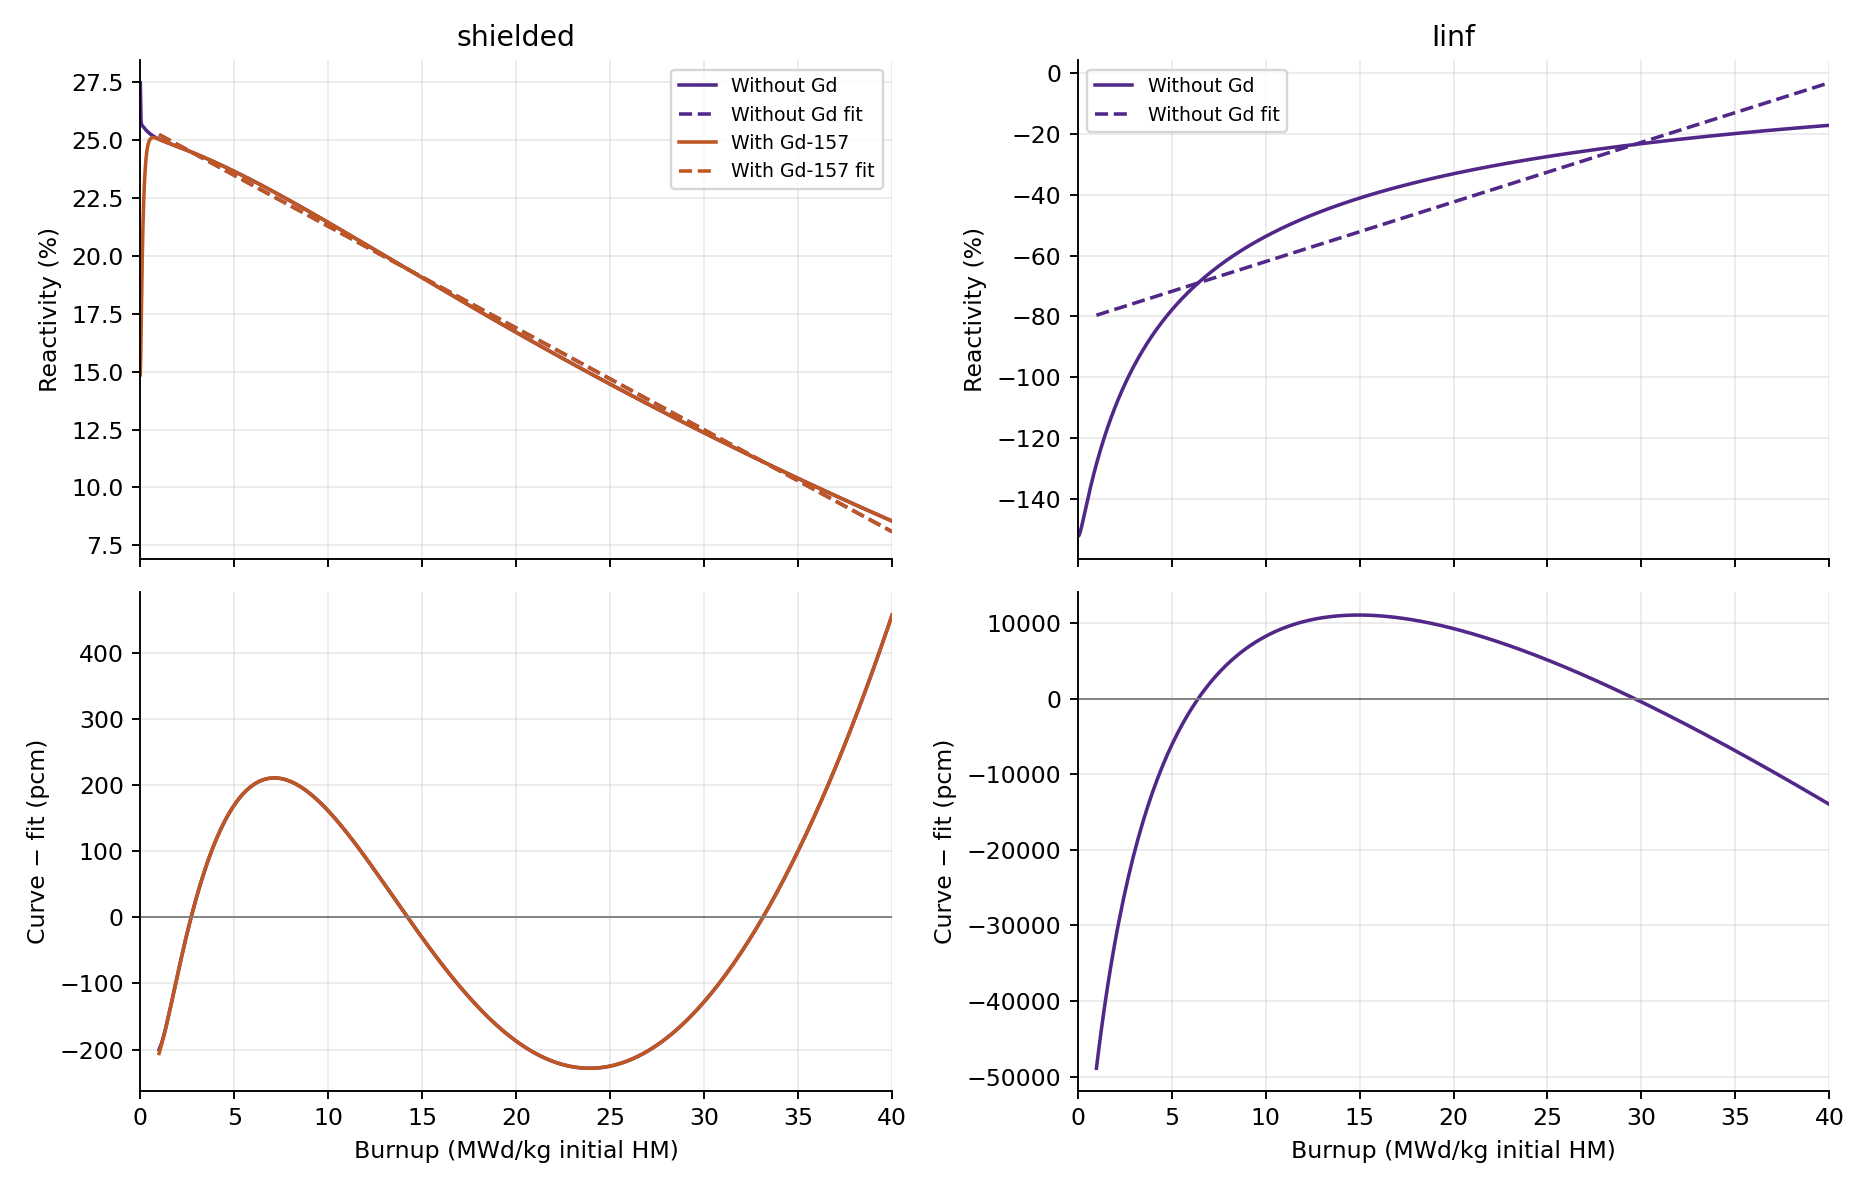
\includegraphics[width=0.96\textwidth]{hw24_fits.png}
\end{center}

\clearpage
\subsection*{(4) Infinite-dilution U-238 and the cycle-length error}
\textbf{Problem.} Use \texttt{xs\_unshielded} in place of \texttt{xs3}
and rerun the non-Gd case. Repeat its part (3) fit and cycle estimate,
and evaluate $\Delta B_c=B_{c,I_\infty}-B_{c,\mathrm{shielded}}$ and
$\Delta t_{\mathrm{days}}=10^6\rho_{\mathrm{HM},0}\Delta B_c/300$.
Check units and use the cycle difference, not the discharge difference.
Assume one operating day at Wolf Creek earns exactly \$1 million gross
revenue; report $L_{\mathrm{million\ dollars}}=\max(0,-\Delta t)$,
or unsupported promised days if the cycle is overestimated.

\begin{draftsolution}
The assigned shielding correlation gives
\[
 I_{\mathrm{shielded}}=4.45+26.6\sqrt{\frac{4}{10.4(0.82)}}
 =22.66747\ \mathrm b,
 \qquad I_\infty=278\ \mathrm b.
\]
These are effective intermediate-group absorption integrals; their ratio
is about 12.26. The corresponding one-group non-fission U-238 absorption
cross sections are about 1.34482 and 13.54258 b, respectively, because
the fast and thermal terms are retained. The assignment's code change
also scales the tiny intermediate-group U-238 fission integral, as
implemented in \texttt{three\_group\_xs}.

Extra U-238 capture initially imposes a large neutron loss and then feeds
U-239 $\to$ Np-239 $\to$ Pu-239. At 3.5 years, the no-Gd shielded
Pu-239 density is approximately $2.25945\times10^{20}$ atoms/cm$^3$,
while the altered model gives $1.47944\times10^{21}$ atoms/cm$^3$.
The enhanced breeding increases fission production, so the altered
fixed-power flux falls to $5.46496\times10^{13}$ n/cm$^2$/s.
These inventory changes require new depletion solves; a final balance
with changed cross sections alone would not reproduce them.

The altered non-Gd case initially has $\rho=-1.505267$, corresponding
to $k$ near 0.399.
Reactivity below $-1$ is mathematically allowed by $\rho=1-1/k$.
Its reactivity remains negative throughout the available history. Its rising
post-startup fit has $a\simeq-0.01959<0$ and
$\rho_0\simeq-0.81545<0.05$. The decreasing-reactivity cycle assumptions
both fail. The positive formal $B_c\simeq22.09$ is produced by dividing
two negative numbers; it has no valid cycle interpretation. This rising curve does not describe
an initially operable, depleting equilibrium cycle.

Subtracting the shielded non-Gd formal cycle estimate nonetheless gives the
requested arithmetic:
\begin{center}\small
\begin{tabular}{lrrr}
\toprule
BP case & $\Delta B_c$ & $\Delta t$ (days) & Formal $L$ (\$M) \\
\midrule
Without Gd & -1.4303 & -43.704 & 43.704 \\
\bottomrule
\end{tabular}
\end{center}

Here
\[
 \Delta t=\Delta B_c\frac{10^6\rho_{\mathrm{HM},0}}{P^{\prime\prime\prime}}
 \quad\left[
 \frac{\mathrm{MW\,day}}{\mathrm{kg}}
 \frac{\mathrm{kg}}{\mathrm{cm^3}}
 \frac{10^6\ \mathrm{W/MW}}{\mathrm{W/cm^3}}
 =\mathrm{day}\right].
\]
The sign is negative: the blind formula underestimates the formal cycle
by about 43.70 days, or \$43.70 million under the stipulated gross-revenue
conversion. It is the \emph{cycle} burnup difference; using the discharge
difference would introduce a factor-of-three error.

\textbf{Interpretation.} This
dollar figure is formal arithmetic from an invalid altered model, and
even the shielded limiting discharge extrapolates outside the history.
It establishes neither a defensible operating schedule nor an actual
financial loss. The imposed-power ODE can integrate a subcritical state;
it does not supply the missing source or prove self-sustained operation.
\end{draftsolution}
\begin{center}
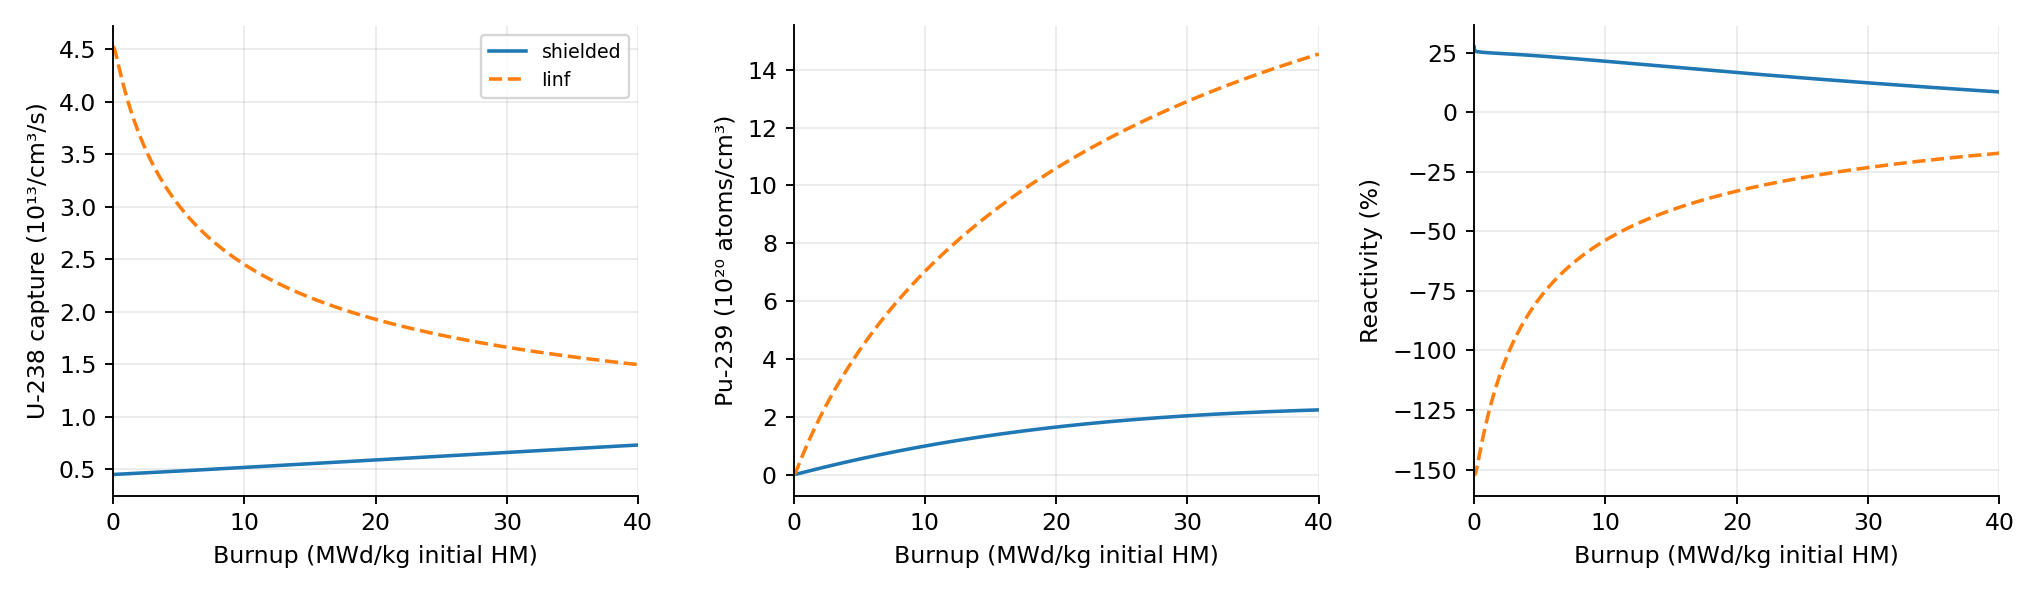
\includegraphics[width=\textwidth]{hw24_cross_section_effect.png}
\end{center}

\clearpage
\subsection*{Additional verification: nonlinear batch-average comparison}
\textbf{Optional instructor check.} This comparison was part of the
earlier draft. It is retained as numerical evidence and is not an
additional requirement of the revised assignment.

\begin{draftsolution}
For the proposed cycle, the actual core approximation is
\[
 \rho_{\mathrm{core}}(b)=\tfrac13\sum_{j=0}^2
 \rho_\infty(10j+b)-0.05,\quad 0\le b\le10,
\]
whereas the linear approximation is
$\rho_{\mathrm{core,LRM}}(b)=\rho_0-0.05-a(10+b)$.
\begin{center}\small
\begin{tabular}{lrrrr}
\toprule
Case & Curve BOC & Curve EOC & LRM BOC & LRM EOC \\
\midrule
Shielded, no Gd & 0.168662 & 0.118298 & 0.162754 & 0.118810 \\
Shielded, Gd & 0.126639 & 0.118298 & 0.162753 & 0.118809 \\
$I_\infty$, no Gd & -0.841058 & -0.416646 & -0.669536 & -0.473626 \\
\bottomrule
\end{tabular}
\end{center}

For shielded fuel without Gd, the nonlinear core reactivity decreases
from 0.168662 to 0.118298. For shielded fuel with Gd, it starts at
0.126639, rises to about 0.158916 near $b=0.541$ MWd/kg
(16.52 days into the cycle), and then falls to the same EOC value.
This rise is about 3228 pcm above its own BOC. The nearly identical
post-startup LRM lines miss the fresh-batch poison transient: their
Gd-case BOC is about 3611 pcm too high. They also miss the intermediate
peak. Reporting only BOC and EOC would conceal this failure.

At the shielded LRM-predicted EOC, the 47.04 and 70.55 MWd/kg batches
are outside the history. The nonlinear EOC residual is therefore
\textbf{unsupported}, rather than zero or an endpoint-clamped value.
The same issue affects the unshielded non-Gd case, whose formal EOC burnups
are approximately $(22.09,44.18,66.26)$ MWd/kg. All three EOC residuals
are deliberately blank in the numerical evidence.

The fixed-power histories have no downward zero-reactivity crossing in
the simulated shielded range. The 10 MWd/kg curves retain positive
uncontrolled excess at EOC, but that observation does not validate a
70.55 MWd/kg discharge extrapolation or establish controllability. No
nonlinear operating-cycle length has been inferred outside the history.
\end{draftsolution}
\begin{center}
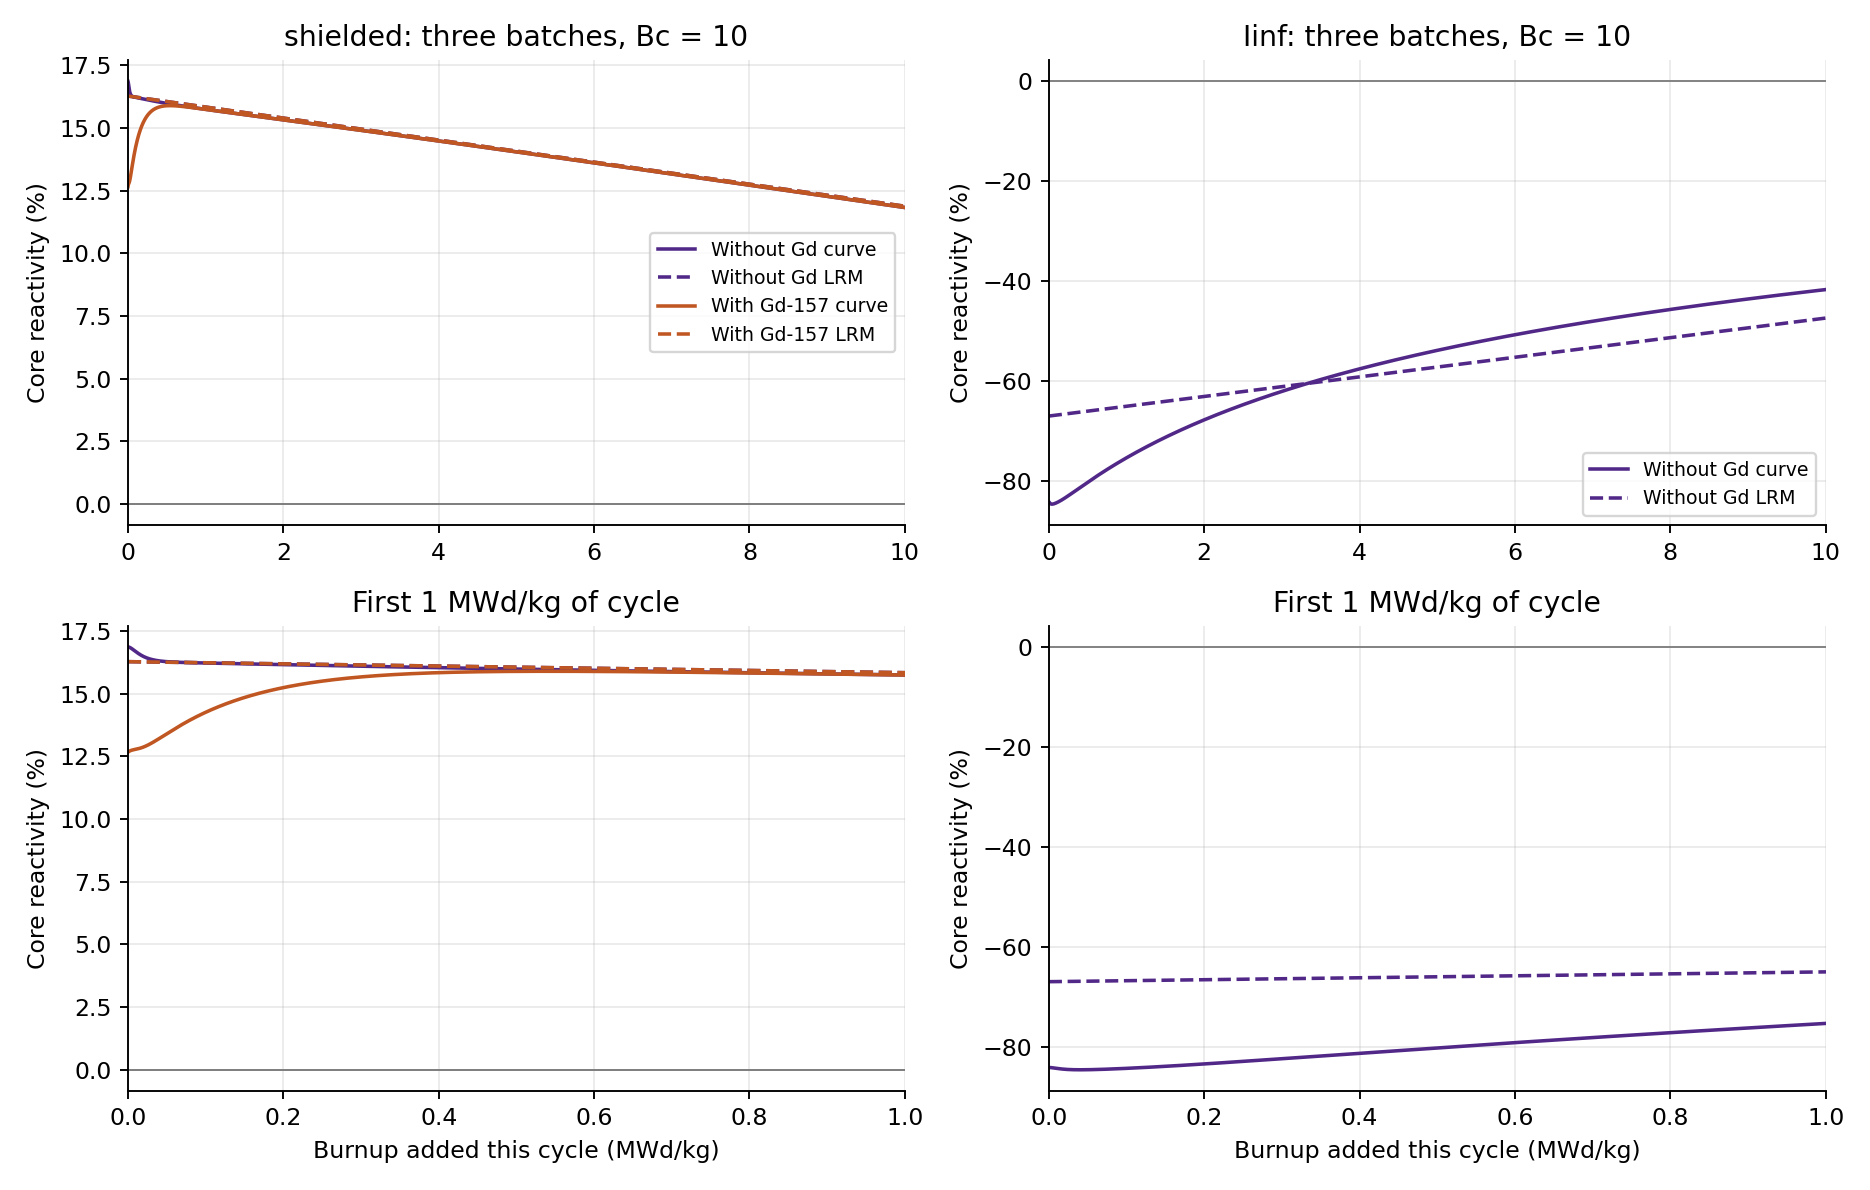
\includegraphics[width=0.96\textwidth]{hw24_core10.png}
\end{center}

\subsection*{Verification and remaining limits}
The numerical builder fails if any required check fails. It verifies
power by an independently assembled fission balance, initial HM mass
from the enrichment formula, burnup from integrated energy, reactivity
from independently summed fuel/moderator production and absorption,
analytic Gd depletion and Gd-to-sink atom conservation, and independence
of the actinide histories from Gd in this fixed-spectrum model.
It repeats each calculation with tighter BDF tolerances, a doubled output
sampling density, and the independent Radau integrator. It also rejects
out-of-range interpolation explicitly.

The retained verification table quantifies integration and sampling
errors separately. At the reference sampling density, doubling output
density changes reported core extrema by less than 0.1 pcm; the coarser
starter grid can shift the Gd-bearing core peak by about 1.65 pcm.
The independent solvers agree much more closely than the fit residuals.
These checks verify the solution to the specified teaching equations.
The prescribed spectrum, approximate data, omitted Gd spatial
self-shielding, incomplete chain, equal batch weights, and absence of
feedback or explicit control remain model limitations.
